\chapter{評価実験}
\label{chap:experiment}

本章では、本論文で提案する『わかるらんど』の研究室での利用実績や
WISS2016での評価実験について述べる。

\newpage

\section{研究室においての利用実績}
我々の研究室では,
約6ヶ月の間『わかるらんど』を研究室内の大型ディスプレイに表示して実際に利用してきた.
我々の研究室ではWebLindaを使用して,
Web情報やArduinoやRaspberry Piに接続したセンサ情報を利用し,
\begin{itemize}
\item 部屋の明るさを知る
\item 部屋の温度を知る
\item 風速と風向を知る
\item 入口のドアの鍵を開ける
\item 部屋の照明を点ける/消す
\end{itemize}
といったことをSlack\footnote{https://slack.com}のチャットボットを通じて行える
IoT環境を構築している(図\ref{slack})が,『わかるらんど』と組み合わせることで
さらに便利に使うことができた.

\begin{figure}[h]
\centering
\fbox{
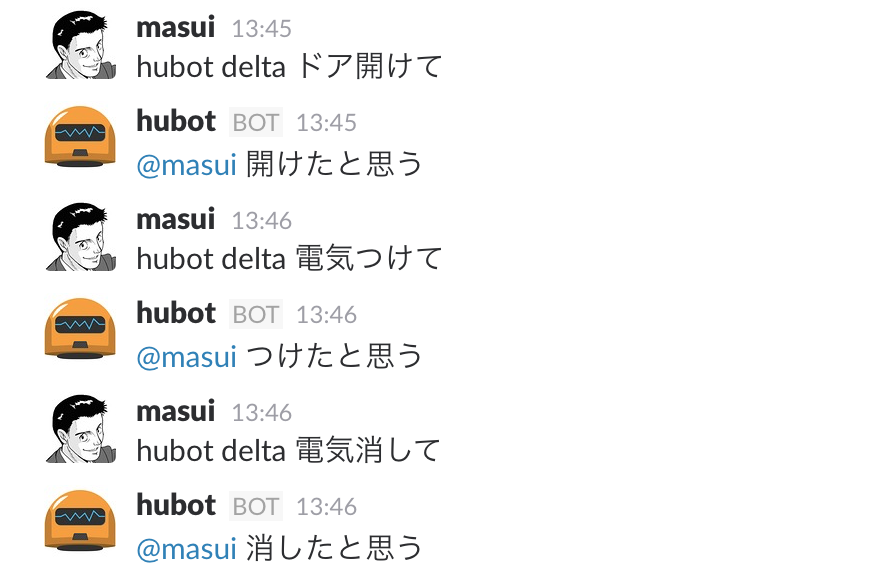
\includegraphics[width=9cm]{images/slack.png}
}
\caption{SlackのチャットボットによるIoT機器の操作}
\label{slack}
\end{figure}

図\ref{light}は部屋の明るさを表示するデータセルだが,
明るさのデータの値が小さい時は\texttt{background}画像を変更することで,
照明が点いているのか消えているのかがわかるようになった.

\begin{figure}[h]
\centering
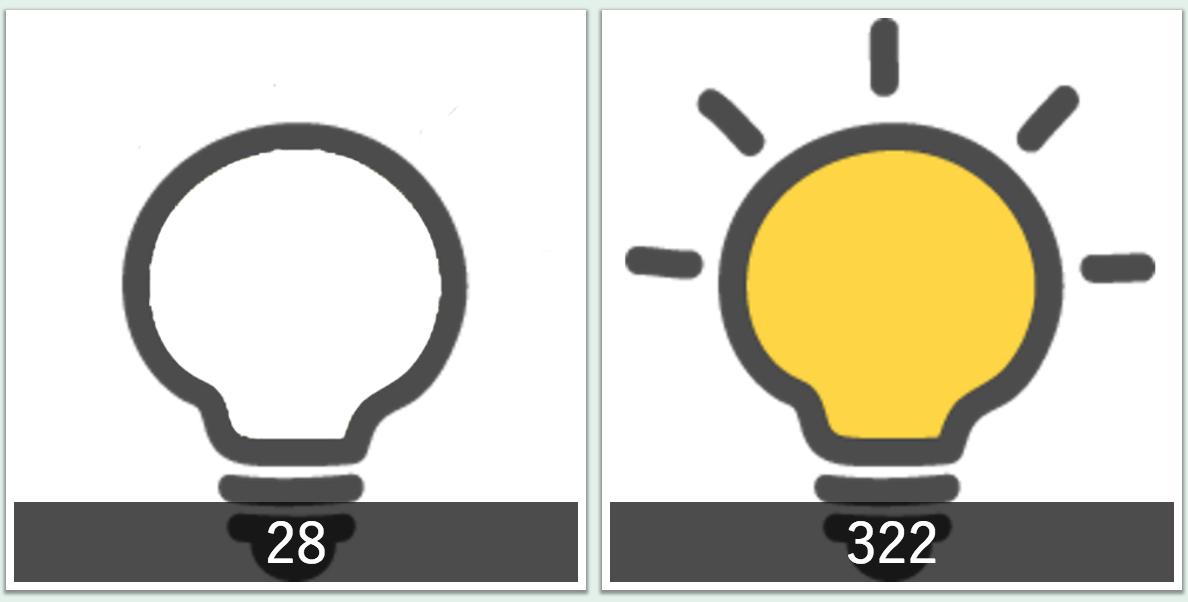
\includegraphics[width=9cm]{images/light.png}
\caption{照明が消えている時(左)と点いている時(右)}
\label{light}
\end{figure}

図\ref{door}は,研究室のドアが最後に開いた時間を表示するデータセルである.
普段は扉の画像を\texttt{background}にしているが,
実際に扉が開いた時に10秒間だけ\texttt{background}を図\ref{door}右のように
扉を開ける人の画像にすることで,誰かが入室したことが視覚的にわかるようになった.

\begin{figure}[h]
\centering
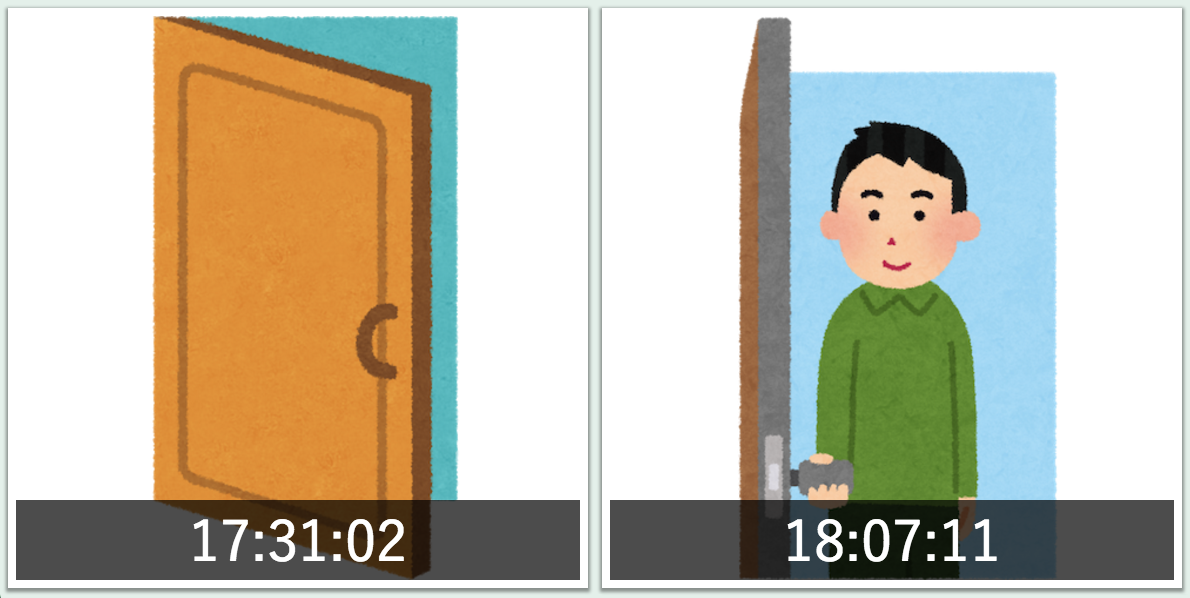
\includegraphics[width=9cm]{images/door.png}
\caption{ドアの普段の表示(左)と誰かが入室した時(右)}
\label{door}
\end{figure}

ミーティングの時間には積極的に『わかるらんど』を利用し,
普段発言の少ない人でも何らかの反応を表明したり,
発表者が聴衆の反応をひと目で把握することができるようになった.
発表中に『わかるらんど』に「わからん」というリアクションが並んだときは,
発表者が詳しい説明をすることができたり,
誰かが面白いことを言ったときに「笑」というリアクションが並び,
『わかるらんど』を通じて一体感が生まれたりすることもあった(図\ref{wara}).

\begin{figure}[h]
\centering
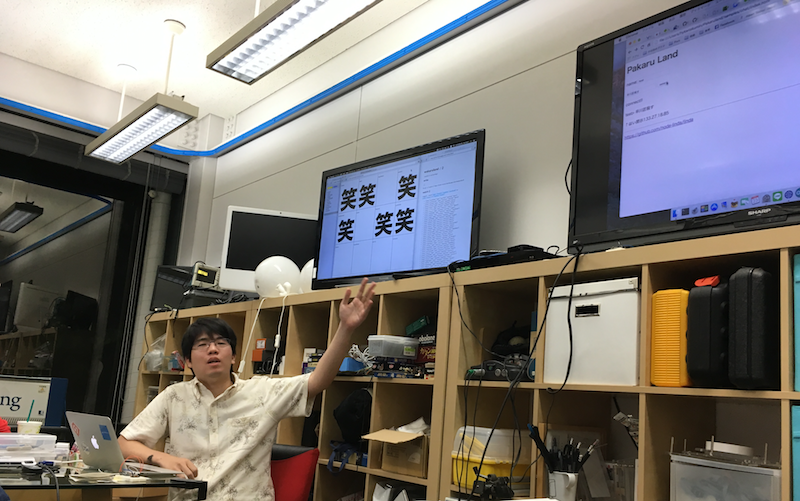
\includegraphics[width=9cm]{images/wara.png}
\caption{『わかるらんど』を使用したミーティング}
\label{wara}
\end{figure}

また,コンピュータで何か別の作業をしているときに,
Webブラウザで『わかるらんど』を開いてリアクションするのが面倒であるという意見もあった.
そこで,図\ref{heebutton}や図\ref{10key}のような
独自の『わかるらんど』入力ハードウェアを作成した.
これらを利用することで,限られたリアクションではあるが,
Webブラウザを開くことなく『わかるらんど』にリアクションを表示することができるようになった.

\begin{figure}[h]
\centering
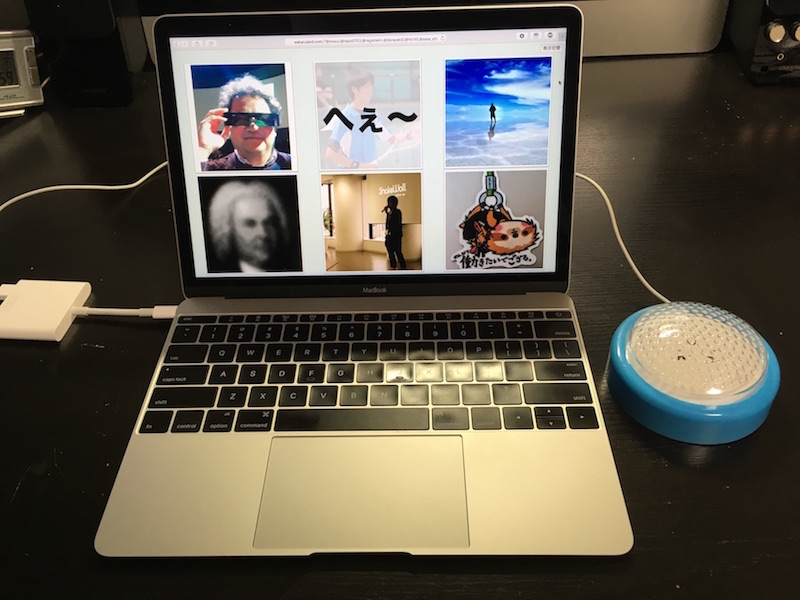
\includegraphics[width=8cm]{images/heebutton.png}
\caption{押すと「へぇ〜」とリアクションできるボタン}
\label{heebutton}
\end{figure}

\begin{figure}[h]
\centering
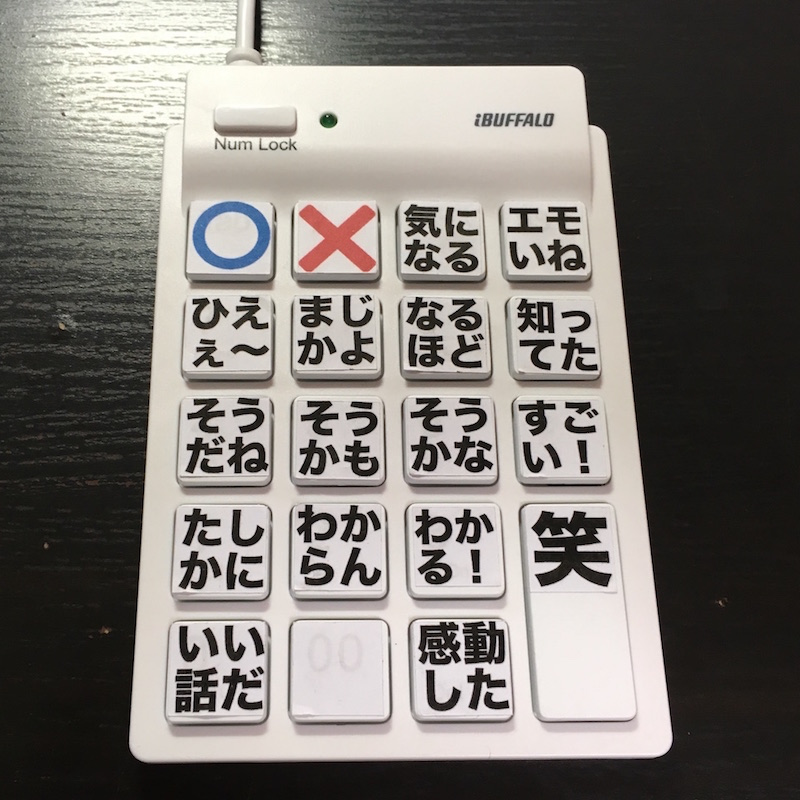
\includegraphics[width=7cm]{images/10key.png}
\caption{テンキーを利用した入力装置}
\label{10key}
\end{figure}

\clearpage


\section{WISS2016での実証実験}
WISS2016において、プレゼンテーションセッション、デモ中継セッション中のコミュニケーションシステムとして
3日間『わかるらんど』を運用する実証実験を行った。
WISS2016では運営が用意したチャットシステム「On-Air Forum」と『わかるらんど』の
2つのコミュニケーションシステムが同時に運用された。
On-Air ForumはWISSここ数年続けて利用されており、
『わかるらんど』は今回が初めての運用であった。
会期中に全参加者の半数弱にあたる72人が『わかるらんど』で少なくとも1回発言した。

\subsection{運用デザイン}
WISS2016では、プレゼンテーションセッション会場の前方に3つのつの大型スクリーンが用意され、
中央のスクリーンを登壇者の発表スライドの表示に、
左のスクリーンをWISS運営が用意したチャットシステムOn-Air Forumの表示に、
右のスクリーンを『わかるらんど』の表示に使用された(図\ref{wiss2016})。
参加者は持参したノートPCから『わかるらんど』にアクセスし利用を行った。
会期の半分にあたる2日目の午前までは通常通り『わかるらんど』を運用し、
2日目の午後からはアカウント名を隠し匿名で投稿する形に変更し運用を行った。

\begin{figure}[h]
\centering
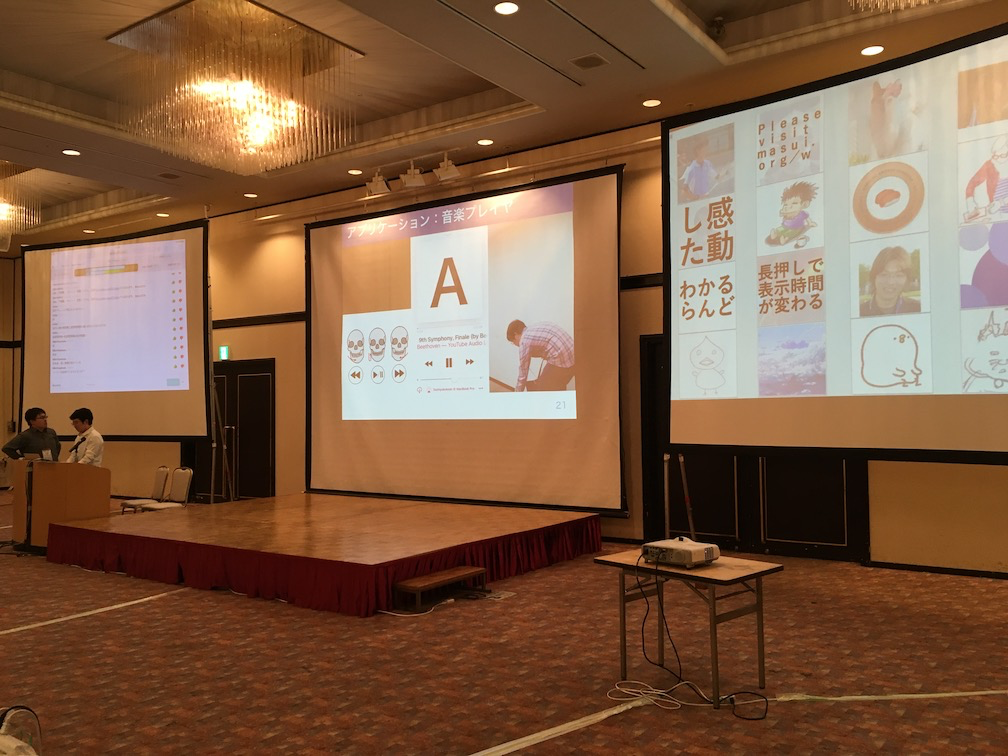
\includegraphics[width=9cm]{images/wiss2016.png}
\caption{WISS2016会場のスクリーン}
\label{wiss2016}
\end{figure}


\subsection{実験の評価指針}
WISSではこれまでにもさまざまなコミュニケーションシステムが運用されてきた。
しかし、各システムの運用成果報告は一部参加者のコメントを掲載するだけであったり、
システムの各機能が実際にどのように使われたかを観察した結果をまとめたものであったりするなど、
コミュニケーションシステムの定量的な評価手法は確立されていない\ref{nishida2006}\ref{nishida2011}。

今回の運用では、今までWISSで運用されてきたコミュニケーションシステムの運用成果報告と同じく、
『わかるらんど』がどのように利用されたのかを観察した結果をまとめるのに加えて、
定量的な評価としてOn-Air Forumと『わかるらんど』の投稿数を比較した。
学術会議には幅広い年齢層・背景の人が参加するため、
親しい者同士のコミュニケーションよりも精神的な敷居が高くなる。
第3章で述べたように『わかるらんど』のコミュニケーションシステムとしての設計指針は
アウトプットを増やすことであり、
アウトプットと同義である投稿の数を増やすことは本システムの評価に極めて重要である。